%%% Local Variables: 
%%% coding: utf-8
%%% mode: latex
%%% TeX-engine: xetex
%%% End:
\documentclass[a4paper,12pt]{article} 

%\usepackage[hmargin=2.25cm, vmargin=1.5cm]{geometry} % Document margins
\usepackage[right=2cm, left=2cm,bottom=2cm,top=2cm]{geometry}

\usepackage[usenames,dvipsnames]{xcolor} % Allows the definition of hex colors
\definecolor{linkcolor}{HTML}{506266} % Blue-gray color for links
\definecolor{shade}{HTML}{F5DD9D} % Peach color for the contact information box
\definecolor{text1}{HTML}{FF0000} % Main document font color, off-black
\definecolor{headings}{HTML}{701112} % Dark red color for headings
% Other color palettes: shade=B9D7D9 and linkcolor=A40000; shade=D4D7FE and linkcolor=FF0080

\usepackage{polyglossia}
\setmainlanguage[variant=uk]{english}

\usepackage{fontspec,xltxtra,xunicode}
\defaultfontfeatures{Ligatures=TeX}
\defaultfontfeatures{Mapping=tex-text}
\setromanfont[Mapping=tex-text,SmallCapsFeatures={Scale=1.1},Numbers=OldStyle]{Optima}%{Adobe Garamond Pro} %{Hoefler Text} % Main document font
\setmonofont[Scale=0.85]{Menlo}

\newfontfamily\descitemfont{Optima}
%\newfontfamily\notefont{Lucida Handwriting}
\newcommand\descitem[1]{{\notefont #1}}
\newcommand\descitemcol[1]{{\color{headings}\descitemfont #1}}

\newenvironment{vlist}[1]{%
\begin{list}{}{%
    \settowidth{\labelwidth}{\tt #1 }     %longest label length
%    \addtolength{\labelsep}{3ex}          %extra space between lbl/txt
    \setlength{\leftmargin}{\labelwidth}  %determine leftmargin
    \addtolength{\leftmargin}{\labelsep}  %determine leftmargin
    \setlength{\parsep}{0.5ex plus 0.2ex minus 0.2ex}
    \setlength{\itemsep}{0.3ex}
    \renewcommand{\makelabel}[1]{\color{headings}\tt ##1 \color{text1}\hfill}}}%
{\end{list}}
%

\usepackage{setspace}
%\onehalfspacing
%\setstretch{1.16}%onehalf is 1.25/1.213/1.241 for 10/11/12 pt
\setstretch{1.10}

\usepackage{titlesec} % Allows creating custom \section's
% Format of the section titles
\titleformat{\section}{\color{headings}
%\scshape%
\descitemfont
\Huge\raggedright}{}{0em}{}[\color{black}\titlerule]
\titlespacing{\section}{0pt}{0pt}{5pt} % Spacing around titles

%\newfontfamily\subsubsectionfont[Color=MSLightBlue]{Times New Roman}
% Set formats for each heading level
%\titleformat*{\section}{\Large\bfseries\sffamily\color{MSBlue}}
%\titleformat*{\subsection}{\large\bfseries\sffamily\color{MSLightBlue}}
\titleformat*{\subsection}{\color{headings}}


\usepackage{enumitem}
\SetLabelAlign{parright}{\parbox[t]{\labelwidth}{\raggedleft#1}}
\setlist[description]{style=multiline,topsep=10pt,leftmargin=2.5cm,font=\normalfont,%
    align=parright}

\newlength{\pdfwidth}
%%\setlength{\pdfwidth}{1.0\textwidth}
\setlength{\pdfwidth}{0.45\textwidth}
\newlength{\halfpage}
\setlength{\halfpage}{0.5\textwidth}
\newlength{\halfpagefig}
\setlength{\halfpagefig}{0.5\textwidth}
\addtolength{\halfpagefig}{-0.25cm}

\newcommand{\fit}[1]{\noindent\resizebox{\linewidth}{!}{#1}}

\usepackage{comment}

\begin{document}

\section*{\Huge{\textbf{SuperSlew}}}
\vspace{1cm}

Plugin that allows you to move your plane around without actually flying.

\vspace{0.5\baselineskip}
It needs X-Plane 10.40+, and works in 32 and 64 bits, on Linux, Mac
and Windows.

\vspace{0.5\baselineskip}
The slew mode can be started and stopped in two ways. First, from the
menu, and second, by binding a key or joystick button to the custom command
defined by the plugin. The command is called
\texttt{durian/superslew/toggle}. 

\vspace{1cm}
\section*{\Huge{\textbf{Installation}}}
\vspace{1cm}

The plugin is distributed as a zip file. The \texttt{superslew}
directory and its contents, contained in the zip file, must be put in
the \texttt{Resources/plugins} directory which can be found in the
main X-Plane directory. The directory containing the plugin
\textsl{must} be called \texttt{superslew}. If installed correctly, a
new menu item called ``SuperSlew'' will appear under the Plugins menu
in X-Plane. This menu contains a number of items. The first one,
called ``Slew Toggle'', switches the slew mode on or off. When
enabled, a small windows containing information is shown in the bottow
right corner of the screen. The following information is displayed.

\begin{figure}[h!]%
\centering
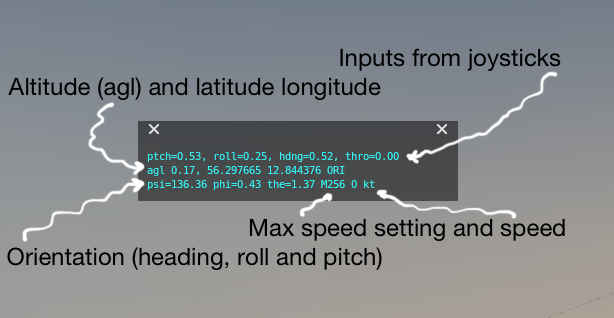
\includegraphics[width=1.0\textwidth]{infowindow.png}
\label{fig:infowindow}
\end{figure}

\vspace{1cm}
\section*{\Huge{\textbf{Controls}}}
\vspace{1cm}

%explain modes first, and what is standard mode

In standard mode, the plane can be moved around with the joystick
and/or pedals. Moving the stick forward or backward will move the
plane forward of backword. The speed at which you move is controlled
by the throttle.

\begin{figure}[h!]%
\centering
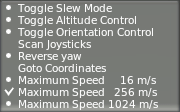
\includegraphics[scale=1]{slewstandard.png}
\label{fig:infowindow}
\end{figure}

\vspace{0.5\baselineskip}
Moving the stick to the right or left moves your plane to the right or
left. If you select the ``Altitude Mode'' from the menu, your plane
will be moved up or down instead. 

\begin{figure}[h!]%
\centering
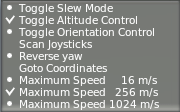
\includegraphics[scale=1]{slewaltitude.png}
\label{fig:infowindow}
\end{figure}

\vspace{0.5\baselineskip}
You can rotate the plane with the pedals (or twist grip on your
joystick). Speed of rotation is controlled by how much you move the
pedals or stick.

\vspace{0.5\baselineskip}
If you switch to ``Orientation Mode'', you can change the pitch and
roll with the joystick. The pedals still change the rotation. This
mode disables the two other modes, so you have to disable it if you
want to move position again.

\begin{figure}[h!]%
\centering
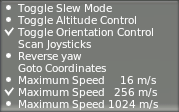
\includegraphics[scale=1]{sleworientation.png}
\label{fig:infowindow}
\end{figure}

\vspace{0.5\baselineskip}
This readme is for version 0.93. 

\vspace{0.5\baselineskip} {\color{text1}This program is shareware. You may try
  it, but if you keep on using it you are encouraged to make a small
  donation. May not be re-distributed, sold or used for commercial
  purposes without explicit permission.}

\end{document}
